\chapter{Of quantities and numbers}
\label{Chapter 1}
\lhead{Chapter 1. \emph{Quantities and numbers}}

\vfill
%\begin{figure}[tbh]
%\centering 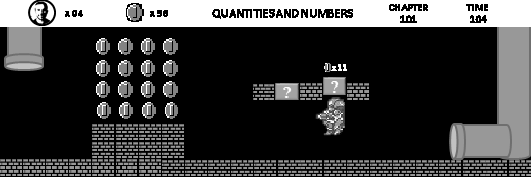
\includegraphics[width = \linewidth]{Figures/ChapterImg/Ch1.pdf}
%\end{figure}
\vfill

\newpage
\section{Thesis overview}
Standing silently in the morning haze, you wait to buy a coffee. Before you are two queues, either of which will lead to a glorious brew. But which queue contains fewer customers? Joining a queue, you look towards the coffee prices: `small' \$5, `regular' \$5.50, and `academic' \$8. Confused, you check the price again; `academic' \$6. Shrugging off the confusion of `6' and `8', you pay for your coffee and start the day. 

Often in life, we experience situations where we must compare the value of two quantities. These quantities may be physical, for example, two queues of five people, or metaphysical, for example, comparing a single queue to an internally stored representation of `ten people'. Both cases require us to perform a \textit{numerical comparison}. 

How the human brain evaluates and compares two quantities is not well understood. For example, can the brain compare two quantities at the same time? Does this process depend on the number of items in each group? How difficult is this task to complete? And does the presence of a second quantity impact our assessment of the first? Just as we perform numerical comparisons between quantities, we also perform numerical comparisons between numerals. 

When we view a numeral, for example '2', we compare its features to those of our previously stored mental representations, 1, 2, 3..., before identifying the best match. The confusion of one numeral for another reflects similarities between our mental representations. These similarities may be perceptual, for example 3 and 8 look more similar to each other than 3 and 7, or numerical, for example 1 and 2 are numerically closer than 1 and 9. But which plays a larger role in our confusions: our perception, or our internal representation of quantity?

%%AE: because the notion of similarity is tricky, as we have agreed, it'd be best to capture it in RELATIVE terms, as i have done above. I'll mention this again when we talk: be careful with the use of similarity; it is ill defined and quite contentious 


%%AE: below and else where: would either past of present tense be better than future tense? after all you have already done the work...

\subsection{Thesis aim and structure}
The aim of this thesis is to provide new insights into the fundamental cognitive processes that govern our comparisons of quantity and our confusion of numbers. This thesis is broken into two broad research streams: the comparison of quantities and the confusion of numbers. The first research stream examines how the human brain evaluates and compares two groups of items at the same time. The second research stream uses confusion data to examine the mental representations of symbolic numerals (\eg Arabic digits) and non-symbolic numerals (\eg domino tiles). 

This thesis composes eight chapters, structured into two research streams, the comparison of quantity (Chapters 2--5) and the confusion of numbers (Chapters 6--7; illustrated in Figure \ref{fig:ThesisSummary}). Chapter 1 introduces key concepts from both research streams before highlighting the aims of each subsequent chapter. Chapters 2 and 3 examine how we compare and estimate large quantities, and Chapter 4 examines how we compare small quantities. Chapter 5 will provide a theoretical extension to the previous chapters for when participants use a mixture of processing strategies. Chapters 6 and 7 examine the confusion of numbers and the dimensions along which we confuse numerals. Chapter 6 examines numeric confusions within an English speaking cohort, and Chapter 7 examines numeric confusions within a Chinese speaking cohort, before concluding with a cohort comparison. Finally, Chapter 8 will discuss the general conclusions, implications and directions of this thesis.

\begin{figure}[tbh]
\centering 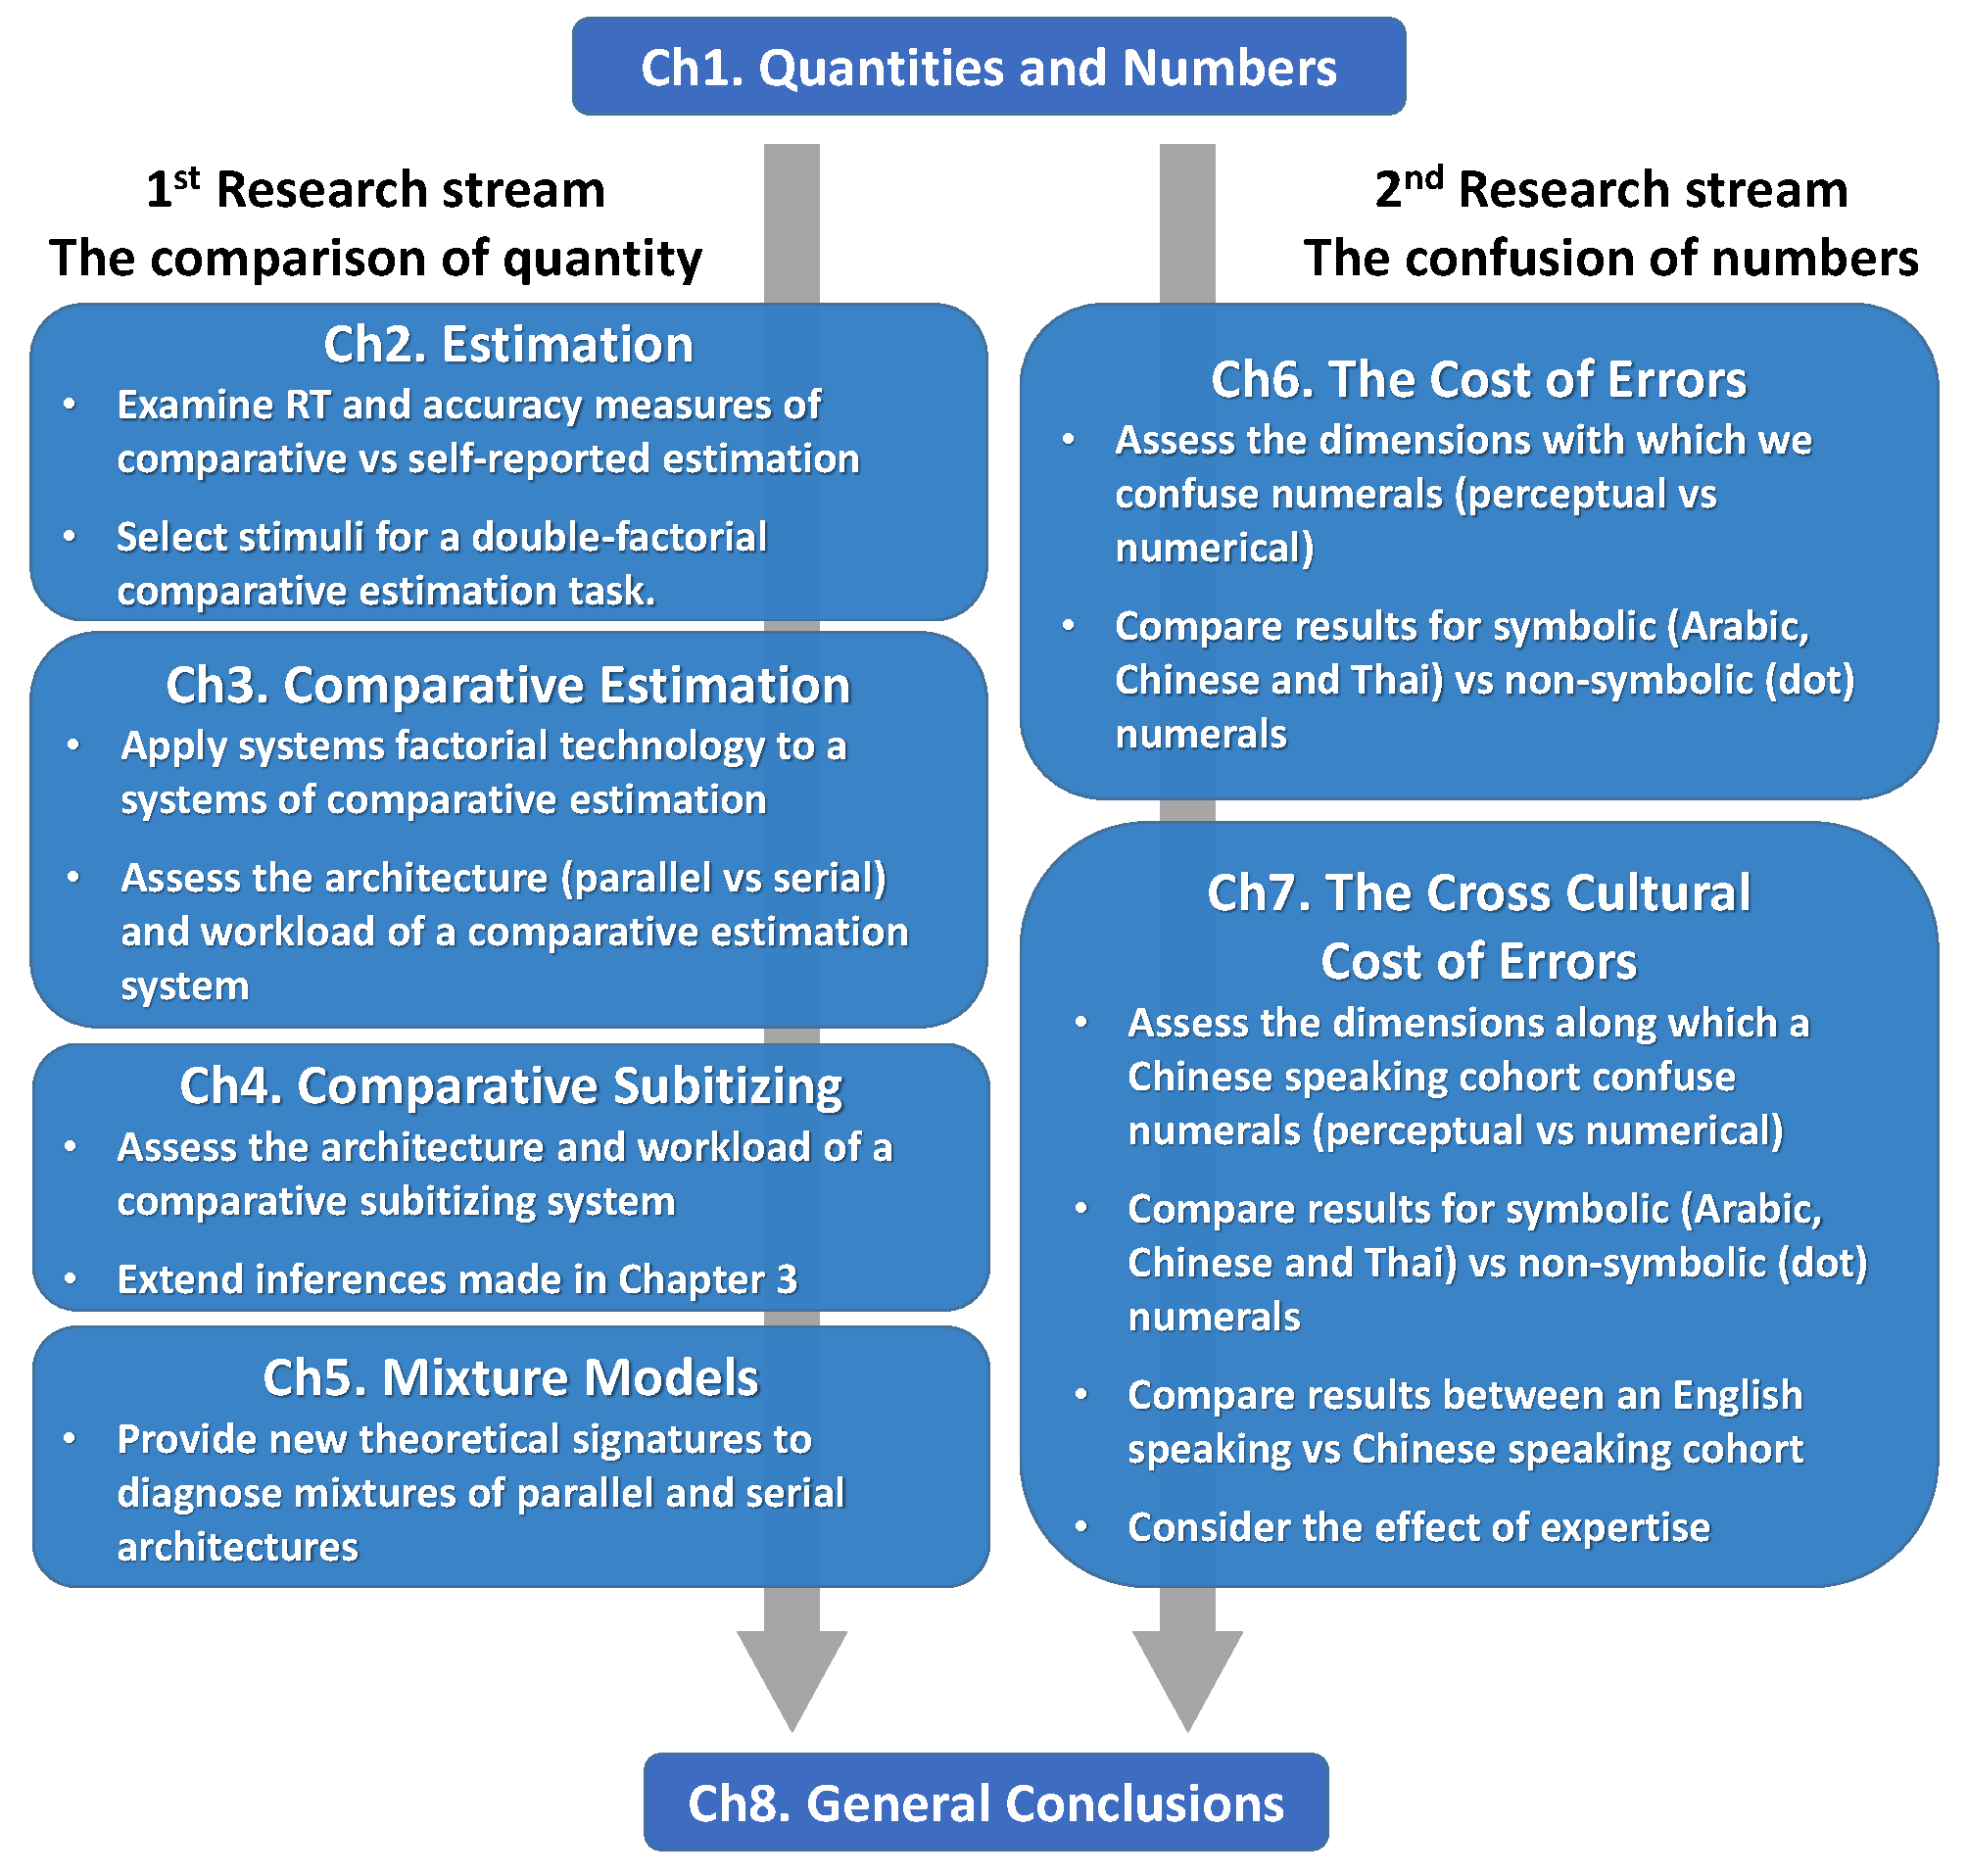
\includegraphics[width = \linewidth]{Figures/Intro/ThesisSummary.pdf}
\caption{Overview of the thesis structure. There are two separate, but related research streams: the comparison of quantity and the confusion of number. The chapters within each research stream follow directly from one another, and both streams fall under the broad umbrella of numerical comparisons.}
\label{fig:ThesisSummary}
\end{figure}


\section{Quantities and numbers}
The ability to quantify a group of numerous items and communicate their value has been critical to the development of human civilization \cite{menninger2013number}. Our collective history of trade, finance, agriculture, warfare and scientific discovery has pivoted upon our ability to quantify items and communicate number. In our modern society, we rely on quantities and numbers to measure time and distance, cook recipes, track social media engagement and perform mathematics. Although less apparent, we rely on quantities and numbers to run our computers and phones, track our money, heat our homes, and secure our electronic identities. Quantities and numbers are instrumental to our everyday lives, and as such, have been studied closely by many cognitive scientists. In the following Chapter, I summarise key concepts and findings from this literature, before expanding on the aims of each thesis chapter\footnote{For the purpose of the introduction and closing chapters, I will use the personal pronoun `I'. The pronoun `we' will be used in the content Chapters to reflect the many contributions of my collaborators.}. 

\section{Quantities}
\subsection{The enumeration of quantity}
\subsubsection{Counting}
Quantities, such as a queue of people, are assigned value through a process of \textit{enumeration}. Counting is one process of enumeration and describes the slow, sequential accumulation of items over time \cite{dehaene2011NumSense}. When we count a quantity, or \textit{item-set}, we unknowingly engaged with five basic principles of counting. 

In their investigation of children's counting, \citeA{gelmanCounting} identified the five principles that must be displayed by a countable number set. A number set must display i) a stable counting order (ordinality), ii) a one-to-one mapping between value and number, iii) cardinality, such that each number is inclusive of previous counts, iv) abstraction, so that counts may generalise to any object, and v) order irrelevance, such that the order an item is counted in does not matter. These basic principles are so complete and universal, they can be used to describe number systems across various human cultures (\eg Arabic, Chinese and Thai numerals).

The process of counting is useful when we wish to know the exact value of an item-set. For example, when we wish to detect the small difference between 14 and 15 apples, or the difference between 21 and 22 dollars. However, often we are less concerned by an exact difference between quantities, and more interested by a relative difference in magnitude. For example, quickly judging that 14 apples are fewer than 20 apples. Such judgements of quantity do not require the slow process of counting, but instead, rely on a different process of enumeration.

%% AE: paul, you use 'upon' extensively (eg rely upon), and i think it'd be good to either replace it with 'on', or at least mix a bit
% PG: Yep, I'll fix this on the read through.

\subsubsection{Estimation}
Estimation is a fast process of enumeration that characterises coarse differences in quantity by changes in relative magnitude. For example, one could estimate that a crowd of 20 people were fewer than a crowd of 30 people, however, one may not be able to estimate that a crowd of 20 were fewer than a crowd of 22. The ability to estimate changes in relative magnitude stems from our innate approximate number system (ANS). %% AE: i added coarse above, otherwise why can you tell apart 20 from 22?
% PG: Sounds great, cheers

The ANS is an inherent system presumably present in many species, including humans and primates \cite{woodruff1981primative}, parrots \cite{pepperberg2005number} and fish \cite{pepperberg2005number}. The ANS, and by extension estimation, requires very few attentional resources \cite{Burr2010} and is capable of simultaneously estimating the number of items within a scene \cite{gallistel1992ANS,dehaene2011NumSense}. This system is responsible for our ability to detect changes in relative magnitude between two quantities.

The ANS follows a logarithmic scale, obeying the Weber-Fechner law, such that detecting a difference between a small quantity and a large quantity depends on their ratio \cite{fechner1860}. For example, detecting a difference between 10 and 20 apples is approximately equivalent to detecting a difference between 20 and 40 apples.\footnote{In other words, when it comes to the ANS it's the proportional difference that `counts'.} This means small differences in quantity are often overlooked. ANS estimates balance the rapid ability to enumerate a quantity, against the inaccuracy of estimation. Although this balance is important when enumerating large quantities, it becomes unnecessary at very small counts.

\subsubsection{Subitizing}
Subitizing is the rapid and very accurate enumeration of 1--4 items \cite{kaufman1949subtizing}. Subitizing, like estimation, is able to quantify an entire item-set simultaneously; however, unlike estimation, subitizing does so without cost to accuracy. The process of subitizing was first described by \citeA[later named by Kaufman et al., 1949]{jevons1871power}\nocite{kaufman1949subtizing} who noticed five or fewer beans could be accurately and simultaneously counted, without conscious attention. The effortless nature of subitizing has led researches to speculate the process may be an innate form of enumeration.

The ability to subitize has been found in human infants \cite{fitzhugh1978role, klein1988universals} and increases from a maximum of two items, to three or four items over the ages of 2--5 \cite{starkey1995development}. The ability to subitize precedes the ability to count \cite{fitzhugh1978role} and is thought to play a role in our early ability to identify one item from a group of two or three similar items \cite{starkey1995development}. Subitizing, unlike estimation, requires attention \cite{Burr2010} and is not derived from the ANS. Rather, subitizing may be derived from the object tracking system.

The object tracking system is an innate perceptual system responsible for distinguishing one item from another and for simultaneously tracking up to four items through space \cite{feigenson2004core, pylyshyn1988tracking}. Although some have suggested subitizing is related to the ANS \cite{dehaene1994dissociable}, it is now generally considered part of this innate object tracking system \cite[but also see Revkin, Piazza, Izard, Cohen, \& Dehaene, 2008]{chesney2011evidence}\nocite{revkin2008does}. 

Subitizing, estimation and counting are three processes through which we may enumerate a single item-set. Often, we enumerate one item-set with the intention of comparing it to another. For example, we may subitize and compare the number of cookies on two plates, or estimate and compare the number of people leaving through two exists at the cinema. But how does the human brain achieve such tasks? For example, do we enumerate one group, then another, and compare them (so-called serial processing), or enumerate and compare both groups at the same time (i.e., in parallel)? 

\subsection{Comparing quantities}
We compare quantities for a variety of reasons. Sometimes we seek to directly compare and match two quantities, for example, matching guests to dinner plates. Other times, comparisons are made to answer a question of inequality, for example, which plate has more cookies? Finally, we may compare one quantity to an internal representation, for example, how many brownies will my friends eat, and will these 10 brownies be enough\footnote{At this stage, it may be apparent that this introduction was written on an empty stomach.}? The way in which we compare two quantities, for example in sequence or simultaneously, can be described in terms of the \textit{processing architecture}.

Processing architecture describes the time course at which information sources are evaluated \cite{Townsend_1995}. A \textit{serial} processing architecture finishes processing one information source (\ie quantity), before starting the next. By contrast, a \textit{parallel} processing architecture evaluates both sources of information at the same time. These descriptions of processing architecture easily extend to our comparisons of quantity.

Comparing two quantities via counting is best described by a serial processing architecture. One item-set must be sequentially enumerated (dotted arrows, Figure \ref{fig:Ch1_CountEstSub}.a), before counting may begin the next (black arrows, Figure \ref{fig:Ch1_CountEstSub}.a). Estimation and subitizing are not accumulative processes and can simultaneously enumerate a single item-set (e.g., dotted lines, Figure \ref{fig:Ch1_CountEstSub}.b). Therefore, it may be theoretically possible for two item-sets to be estimated (or subitized) and compared at the same time through a parallel processing architecture (e.g., black arrows, Figure \ref{fig:Ch1_CountEstSub}.c). Indeed, recent research indicates this might be the case. 

\begin{figure}[tbh]
\centering 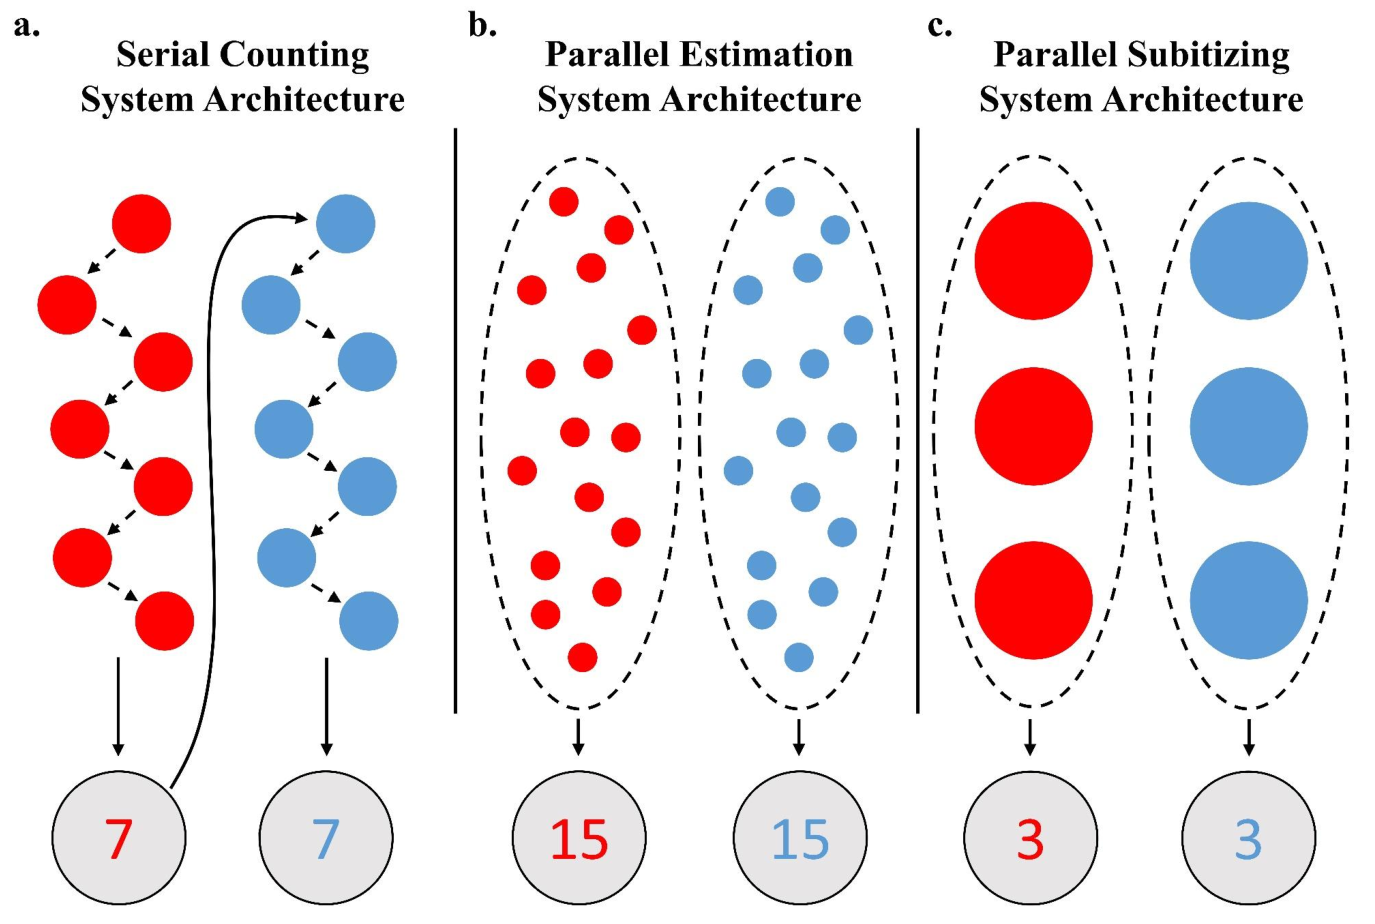
\includegraphics[scale = .65]{Figures/Intro/CountEstSub.pdf}
\caption{a) Illustration of a serial counting system architecture. Note the red-set must be counted first, before counting on the blue-set may begin. b) A theoretical parallel estimation system. c) A theoretical parallel subitizing system. Parallel systems quantify both color-sets (dashed-lines) at the same time.}
\label{fig:Ch1_CountEstSub}
\end{figure}

\subsubsection{Comparative estimation}
In their 2006 study, \citeauthor{HALBERDA_2006} provided the first evidence of a `parallel estimation system'. In this study, participants were presented an array of 1--35 dots, made from 1--6 colors. A color was probed either before or after the stimulus array and participants were asked to estimate the quantity of the probed color-set. If the probe was presented \emph{before} the stimulus array, participants had to estimate the target color-set and report the value with a number-pad. However, if the probe was presented \textit{after} the stimulus array, all color-sets had to be estimated and later, the probed color-set reported. \citeauthor{HALBERDA_2006} found estimation acuity was stable between pre- and post-probe conditions for three or fewer color-sets. Subsequently, \citeauthor{HALBERDA_2006} concluded three or fewer item-sets could be estimated at any one time through a parallel processing system. 

\citeA{HALBERDA_2006} concluded in favor of a parallel estimation system and suggested in their discussion the existence of a parallel subitizing system. As illustrated in Figure \ref{fig:Ch1_CountEstSub}.c, a parallel subitizing system would quantify two small item-sets (each item-set less than five) at the same time. Although \citeA{HALBERDA_2006} provides the first description of a parallel subitizing system for multiple item-sets, the existence a parallel subitizing system has been alluded to in other literature.

%%AE: ok here's a tricky point: parallel processing of multiple sets, as opposed to within set. I added it above and need to be careful in subsequent sections
% PG: Yep, always tricky. Thanks

\subsubsection{Comparative subitizing}
In their investigation of children's numeracy, \citeA{starkey2014groupitizing} found children could quantify an array of items faster, if the items were arranged into groups of 1--4 units. For example, an array of nine items would be enumerated faster if the array were organized into three groups of three. \citeauthor{starkey2014groupitizing} termed this process `groupitizing'. Although the cognitive architecture of groupitizing was never explored, this response-time (RT) facilitation may point towards a `parallel subitizing system'. To understand the wildly speculative nature of this claim, we must first consider a brief history of response-time modelling and the assessment of processing architecture. 

\subsection{Examining processing architecture}
Since the advent of \citeA{donders1868schnelligkeit} subtraction method, response-times have been used to make inferences about human cognition. It was \citeA{egeth1966parallel} who first used response-times to infer differences between parallel and serial processing systems. \citeauthor{egeth1966parallel} assumed that if all items within an array were processes simultaneously (\ie in parallel), the addition of further items would have no impact on decision-time. As such, a parallel system would predict a flat mean RT slope over increasing array sizes. By contrast, a serial system would predict a steep mean RT slope, increasing with arrays size. 

As an early adopter of this method, \citeA{sternberg1966high} applied these principles to examine whether short-term memory was accessed in serial or in parallel. In his task, participants were presented a list of digits followed by a probe, and were asked to report whether the probed digit was in the memory list. \citeA{sternberg1966high} found that response-times increased linearly with the length of the memory list. This `additivity' was used as evidence of a serial processing system, a claim propagated by many influential studies \cite<e.g.,>{Sternberg_1969, cohen1973hemispheric, Shiffrin1977, treisman1980feature}. However, all of these claims ignored the potential for model mimicry.

In the context of processing architectures, model mimicry describes how a slow parallel system architecture may mimic the mean response-times of a fast, serial system architecture \cite<see>[for a case study and review of this topic]{townsend2004serial}. The efficiency at which information sources are evaluated can be described in terms of workload capacity. A limited workload capacity system slows with additional sources of information (e.g., a second item-set), an unlimited workload capacity system is unaffected by additional sources of information, and a super-capacity system speeds up with additional sources of information. The mean RT predictions of \citeA{egeth1966parallel} and \citeA{sternberg1966high} only hold under the assumption of unlimited workload capacity, as a limited capacity parallel system could mimic the mean RT of an efficient serial system. To address this problem of model mimicry, James Townsend and colleagues \cite{Townsend_1995, Townsend_2004, townsend2011} have developed a theoretically driven framework and suit of mathematical tools, known as Systems Factorial Technology (SFT).

\subsection{Systems factorial technology}
SFT is a theoretical framework, augmented by experimental methodology, that uses response-time distributions to specify predictions of unique system-models. By comparing these theoretical models to experimental data, SFT is able to identify system properties without the confound of model mimicry. Specifically, SFT was designed to identify and assess the system properties of architecture, workload capacity, stopping-rule and channel (in)dependence.

Architecture describes the time-course at which information channels are combined (parallel vs serial) and workload capacity describes the system efficiency (limited, unlimited and super). Stopping-rule describes how and when processing may terminate. A self-terminating or minimum-time stopping-rule may terminate before all sources of information are fully processed (e.g., you may terminate your search for a cookie at the moment of its detection). An exhaustive or maximum-time stopping-rule must process all sources of information before a decision can be reached (e.g., you must check all the cookie's ingredients for your friend's nut allergy; see Figure \ref{fig:Ch1_ProcessingChannels}). Finally, channel (in)dependence describes whether information channels are stochastically separate. Independent channels provide no information to one-another. Dependent channels share information and may act to facilitate or inhibit the decision process \cite<see>{eidels2011}. A coactive model describes a special case of parallel processing, where information channels sum together to reach a decision (bottom panel, Figure \ref{fig:Ch1_ProcessingChannels}). Notably, a coactive model is unaffected by stopping-rule and predicts super-capacity. 

\begin{figure}[tbh]
\centering 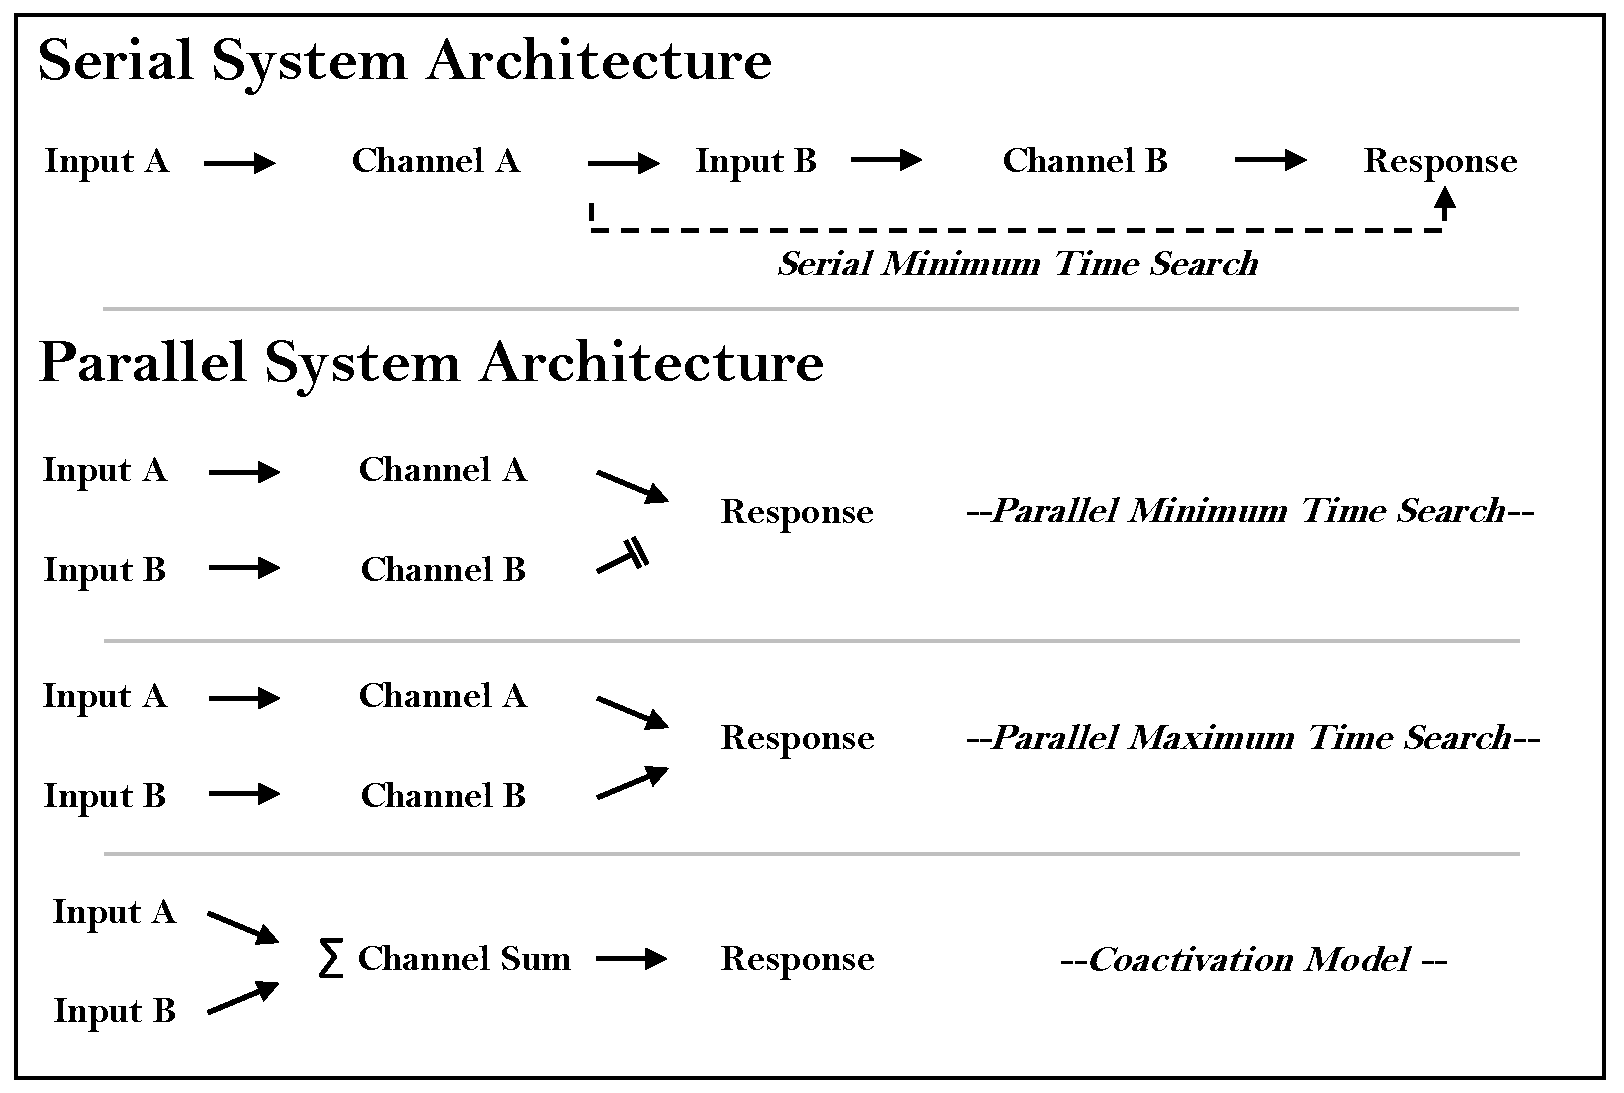
\includegraphics[scale=.54]{Figures/Intro/Architecture.pdf}
\caption{Illustration of parallel and serial processing systems, under minimum-time (self-terminating) and maximum-time (exhaustive) stopping rules. A special instances of parallel processing, coactivation, is also illustrated where channel information is summed. Coactivation models are identical under either stopping-rule.}
\label{fig:Ch1_ProcessingChannels}
\end{figure}

\subsubsection{Double factorial paradigm}
SFT is both an analysis tool set and methodological framework. SFT uses distributional analysis tools to directly assess the properties of system architecture, stopping-rule and workload capacity, under the assumption of channel independence. These analysis tools require a specific methodological design, termed the double-factorial redundant-target paradigm (DFP). Figure \ref{fig:Ch1_DFP} illustrates a prototypical DFP using a dot-detection task. Here, a target is defined by any source of light, and may appear in the left (channel A) or right (channel B) location. Load, (\ie the number of information channels), is manipulated by the presence or absence of a target. Within the target conditions exists a second manipulation of target salience, (\ie target discriminability). A high salience (H) target is easier and faster to respond to than a low salience (L) target. Double-target cells are redundant, as either target would constitute a correct `target present' response. Together, these redundant-cells host four combinations of double-target salience: high-high (HH), high-low (HL), low-high (LH) and low-low (LL). The combined manipulation of load (target presence vs absence) and salience (discriminability high vs low) allows SFT to perform independent assessments of system workload and processing architecture. 


\begin{figure}[tbh]
\centering 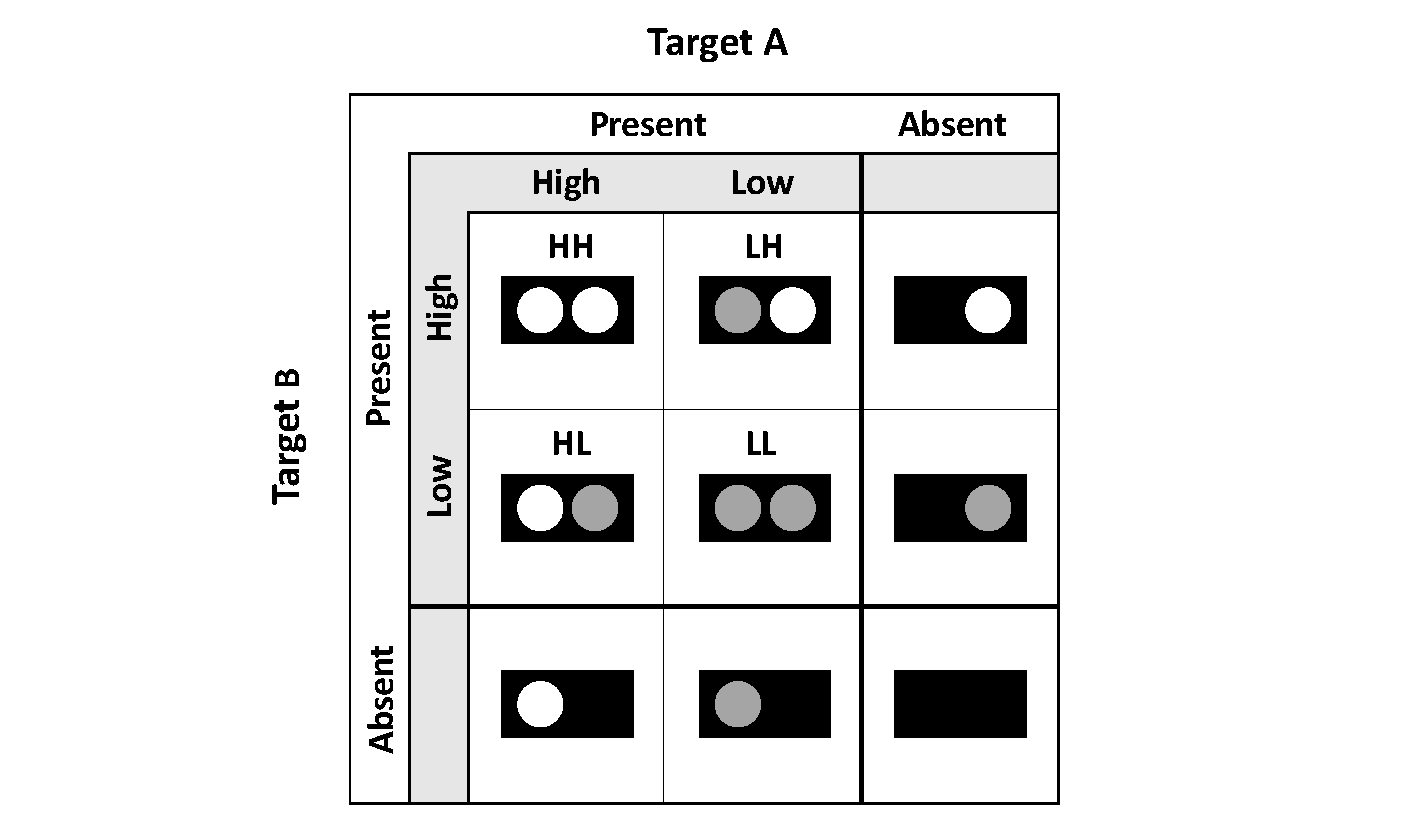
\includegraphics[scale = .6]{Figures/Intro/DFP.pdf}
\caption{Illustration of the double factorial redundant-target paradigm. A `target' is any source of light. One level manipulates workload through the presence or absence of a target. A second level manipulates target salience \ie identifiability --- high (H) or low (L). Two targets are `redundant'; either would constitute a correct target present response.}
\label{fig:Ch1_DFP}
\end{figure}

\subsubsection{Capacity coefficient}
The first factorial manipulation of load allows for calculation of the capacity coefficient [C(\textit{t})]. The capacity coefficient measures the change in efficiency of the processing system as workload, (i.e., the number of information channels), increases. The capacity coefficient is calculated by comparing the response-time distribution for double-target trials, to the response-time distribution for trials when a target is present in each channel alone --- single-target trials. Formally, the capacity coefficient is expressed as:

\begin{equation}
	\rm C(\t) = \frac{\log[S_{AB}(\t)]}{\log[S_{A}(\t)] + \log[S_{B}(\t)]}
    \label{eq:Ct}
\end{equation}

\noindent
where subscript letters refer to the processing channels when each channel operates alone, $A$ or $B$, or together $AB$. $S(t)$ refers to the survivor function\footnote{Throughout this thesis, I use the following notation: $f(t)$, for the probability density function (pdf); $F(t) = \int{f(t)dt}$ for the cumulative distribution function (cdf), and $S(t) = 1 - F(t)$ for the survivor function.} of the channel response-times; $t$ is time, and log is the natural logarithm. The measured change in efficiency between the channel conditions is evaluated against predictions derived from an unlimited capacity independent parallel (UCIP) model. Under the UCIP benchmark model, an unlimited capacity system predicts C($t$) = 1. A super capacity system, one that speeds with additional workload, predicts C($t$) $>$ 1. Finally, a limited capacity system predicts C($t$) $<$ 1. 

\sloppy{
Further predictions for the capacity coefficient have been derived under the purview of the parallel race model. Of particular interest to the current paper is the Grice lower-bound \cite{Grice1984,townsend2011}. The Grice lower-bound is a marker of performance approximately equivalent to serial processing and is formally expressed as:}

\begin{equation}
	\rm C(\t) \geq \frac{\log\{ MIN\, S_A(\t), S_B(\t)\,]\} }{ log[ S_A(\t) \cdot S_B(\t) ] }
    \label{eq:girce}
\end{equation}

\noindent
In a parallel system, violations of the Grice lower-bound suggest severely limited capacity and could be the outcome of channel dependence, where processing in one channel slows the rate of processing in the other \cite{eidels2011}. The Grice lower-bound provides a theoretical comparison by which we can compare parallel system capacity to serial system capacity. 

\subsubsection{Mean and survivor interaction contrasts}
The second factorial manipulation, that of target salience, allows for diagnosis of the system processing architecture through two measures: the mean interaction contrast and the survivor interaction contrast. The mean interaction contrast or MIC, is calculated as a double-difference of mean RT between the four factorial combinations of salience. Formally, the MIC may be written as:

\begin{equation}
	\rm MIC = \left( mRT_{LL} - mRT_{LH} \right) - \left( mRT_{HL} - mRT_{HH} \right)
    \label{eq:mic}
\end{equation}

\noindent
where $mRT$ is the mean response-time, and the subscripts denote the display salience as combinations of high (H; \ie bright dot) and low (L; \ie dull dot) double-target salience-conditions. Thus, HH indicates a trial with two salient targets (\eg two bright dots), HL and LH indicate a trial with one salient and one dull target item, and LL indicates a trial with two dull target items. As high salience targets should be responded to faster than low-salience targets, correct MIC interpretation requires the following ordering: $\rm{mRT}_{\rm HH} < mRT_{\rm HL},\, mRT_{\rm LH} < mRT_{\rm LL}$. Under the assumption of a UCIP model, and correct ordering of the mean RTs, a parallel minimum-time model predicts an over-additive MIC $>$ 0, a parallel maximum-time model predicts an under-additive MIC $<$ 0 and all serial models predict an additive MIC = 0. These three predictions allow the MIC to easily differentiate between parallel and serial models. To further diagnose stopping-rule, we must turn to the survivor interaction contrast (SIC).

The SIC is a contrast measure, similar to the MIC, but calculated from the survivor functions of each double-target salience combination. It is defined as:

\begin{equation}
	\rm SIC(\t) = \left[ S(\t)_{LL} - S(\t)_{LH} \right] - \left[ S(\t)_{HL} - S(\t)_{HH} \right]
    \label{eq:sic}
\end{equation}

\noindent
Different models predict unique SIC($t$) functions, as illustrated in Figure \ref{fig:SIC}. A necessary assumption for valid interpretation of the \SIC is the assumption of selective influence and ordering of the composite salience conditions \emph{i.e.,} $S(t)_{\rm HH} < S(t)_{\rm HL},\, S(t)_{\rm LH} < S(t)_{\rm LL}$. Fortunately, these survivor functions are easily subjected to non-parametric tests. Appropriate application of the \SIC and MIC allows for comprehensive diagnosis of system architecture and stopping rule within the double-target condition.

\begin{figure}[htb]
\centering 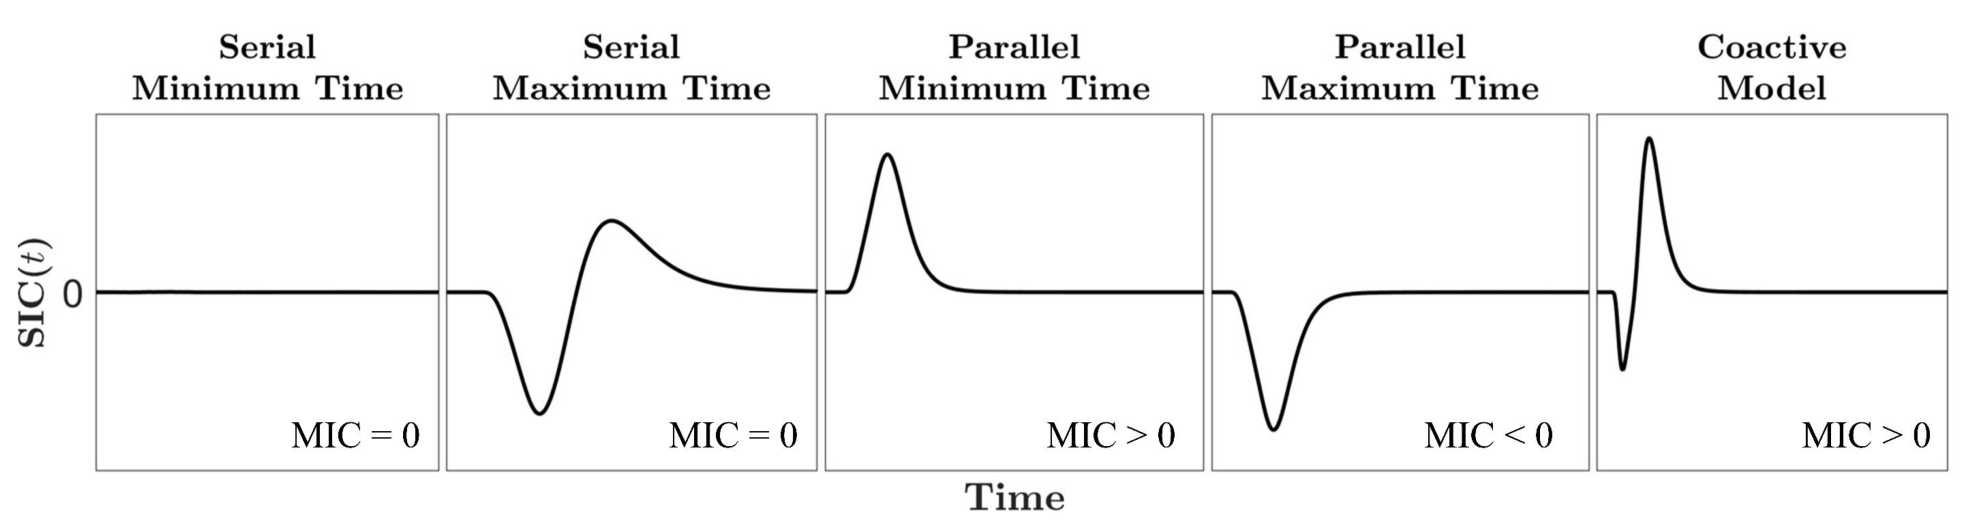
\includegraphics[scale = .47]{Figures/Intro/SIC.pdf}
\caption{Illustration of the five SIC models (and associated MIC values) predicted by the unique combinations of processing architecture and stopping rule. Note, coactivation models are identical under either stopping rule and can be identified by the combination of SIC($t$) and MIC.}
\label{fig:SIC}
\end{figure}

In summary, the distributional tools provided by SFT, once combined with the methodological framework of the double-factorial paradigm, are capable of independently assessing system workload, processing architecture and stopping-rule. This makes SFT the perfect tool-set with which to assess the workload capacity and processing architecture of i) systems of comparative estimation, and ii) systems of comparative subitizing. Now that a firm background has been established regarding SFT, system properties, system measures and comparative enumeration, I present the aims of the first research stream.



\subsection{The comparison of quantity: Chapter aims}
Thus far, I have described three processes of enumeration: counting, subitizing, and estimation, and how these processes are used to compare quantities. I have provided some evidence that two item-sets may be compared through a parallel estimation system, or a parallel subitizing system. I then detailed the issue of model mimicry and why mean RT cannot diagnose parallel and serial processing architectures without accounting for workload capacity. Finally, I described the methodological framework and analysis tools of SFT. Chapters 2--5 focus on the use of SFT and the study of comparative numerosity systems with the following aims.

In Chapter 2 I assess how participants estimate the quantity of a single item-set. The aim of this chapter was to develop a double-factorial comparative estimation task that I later test in Chapter 3. Through experimentation, I select numeric stimuli (i.e., quantities) that fit within the double-factorial framework of load and salience, required for SFT analyses. To do this, I asked participants to estimate a single item-set and report i) their estimation of quantity using a number pad, and ii) their judgement of whether the quantity was less-than a criterion. The results of this study were used to inform the selection of stimuli in Chapter 3. 

In Chapter 3 I implement a double-factorial comparative estimation task using target stimuli selected in the previous Chapter. The aim of this chapter was to assess the processing architecture and workload capacity of a comparative estimation system. To foreshadow, I find evidence of parallel processing architectures, and workload capacity that is so limited, as to be slower than a theoretical serial system. The implications and applications of these findings are discussed.

Chapter 4 extends the work of the previous chapters and develops a double-factorial comparative subitizing task. The aim of this chapter was to assess the processing architecture and workload capacity used for the comparison of small quantities. Here, I find evidence of serial processing architectures operating under severely limited workload capacity. During this chapter, I identify a handful of participants from Chapter 3 and Chapter 4 who display non-prototypical SIC signatures. These participants appear to reflect a mixture of parallel and serial processing architectures.

In Chapter 5 I provide a new set of SIC signatures by simulating and systematically varying the relative proportions of component parallel and serial processing models. These theoretical mixture model are then compared to experimental data to identify participants who displayed a mixture of processing architectures. This process was extended to illustrate the effect of mixture models on the capacity coefficient. Having covered the aims of the first research stream, the comparison of quantities, I now introduce the second research stream: the confusion of numbers.



\section{Numbers}
Quantities can be expressed in a number of ways. Historically, people have used physical markers to represent the count of an item-set, for example, a tally of ten sheep. This method is efficient for small quantities, however, becomes less-efficient and error prone at larger counts. To address this limitation, symbolic numerals were adopted by various cultures and are still used today - for example, Arabic digits. The second research stream of this thesis relates to the numerals we use to symbolically represent quantity. Where the previous research stream investigated the enumeration of an item-set, this research stream will focus on the means of numeric communication.

%%AE: i think more is needed here. Something like: "Quantities could be expressed in various ways. Historically, people used physical markers to represent the number of objects, say, a line for each cow they inteded to exchange. This method could be efficient for small quantities, but with development of commerce they arised the need to represent larger quantities. Symbolic... [say here]. Stand 1 focuses of subitising and estimation with non-symbolic representations. Strand 2 examines the use of symbolic.... 
% PG: Fixed

Human civilisations are shaped by the communication of ideas, emotions and quantities. The ability to accurately communicate quantity has been integral to the advancement of mathematics, finance, agriculture, engineering, and warfare. The importance of accurately communicating quantity has led many cultures to develop their own symbolic numeral systems. For example, the Arabic numerals 0 -- 9 and the Chinese numerals \begin{CJK}{UTF8}{gbsn} 〇 -- 九\end{CJK}. 

Often, when we view one numeral, we confuse its identify with that of another. The cost a confusion varies, and not all confusions are the same. For example, the financial cost of confusing 2 with 3 dollars, is naturally less costly than confusing 2 with 7 dollars. These confusions may be caused by perceptual similarities or numerical proximity. 

The physical similarities between two numerals, for example 2 and 7, or \begin{CJK}{UTF8}{gbsn} 二 and 三,\end{CJK} may lead us to confuse the identify of one numeral for another. The more features shared between two numerals, the higher the likelihood of a confusion. When we identify a numeral, we compare its features with those of our internal mental representations.

Mental representations are theoretical internal cognitive states thought to reflect the external world \cite{mueller2012alphabetic, eidels2016mental}. Items with more similar features are thought to be represented by closer distances within this mental space. For example, the number `2' displays a diagonal midsection and open left-face, and may be confused with the number `7'; this would suggest 2 and 7 are closely aligned along dimensions of perceptual similarity in the mental space. Although the physical properties of numerals may change across cultures, the values they represent do not.
%%AE: oh Blimey, that similarity again. Fine, leave it here [but be careful elsewhere, as i requested]

Numerals maintain the properties of cardinality (unit-value), and ordinality \cite<unique sequential ordering> {dehaene2011NumSense}. With use, these properties become embedded into our internal representation of number; our so called \emph{mental number space}. Numerals are representations of quantity and inhabit the same mental number-space as the approximate number system \cite{dehaene2011NumSense}. This makes numerals subject to basic numerical effects, such as the numerical distance effect.

In the context of numbers, the numerical distance effect describes how numerically-close numbers (e.g., 5 vs 6) are harder to compare than numbers further apart \cite<e.g., 5 vs 9>{moyer1967time}. This displays an effect of proximity between our mental representations of number and means two numerals may be confused due to their numerical proximity. But which plays a larger role in our confusion of numbers: our perceptual representations of number, or our internal representation of quantity? In Chapter 6, I aimed to address this question. 

\subsection{The confusion of numbers: Chapter aims}
In Chapter 6 I assessed the rate at which numerals were confused with one-another in an English speaking cohort. I presented participants with three symbolic numeral types (Arabic, Chinese and Thai numerals) and one non-symbolic numeral type (non-symbolic dots e.g., domino patterns), and asked participants to complete a numeral identification task. Confusion patterns were analysed using multidimensional scaling \cite{shepard1962originalMDS1, shepard1962originalMDS2, kruskal1964nonmetric}, a method used to visualize dimensions of similarity. The analysis was augmented by application of Luce's similarity choice model \cite{luce1963detection} to control for effects of response bias. We find evidence that symbolic numerals were confused (represented) by dimensions of perceptual similarity, and non-symbolic numerals were confused by dimensions of perceptual \textit{and} numerical similarity. 

Chapter 7 extends the work of Chapter 6 within a Chinese speaking cohort. In addition to assessing the dimensions by which numerals are confused, this study provides a new insight into how experience with a numeric-set changes our mental representations. The results of this study were identical to the previous chapter, except that Chinese numerals were represented differently between the Chinese-speaking and English-speaking cohort. These results are discussed in the context of expertise and its effect on our internal representations. 

Finally, Chapter 8 offers a discussion of the general findings and future directions of this research. This chapter will tie together the general conclusions of both research streams: the comparison of quantity and the confusion of number.


% Ami DONE w Intro -- 22/1/2019
